\documentclass[a4paper, 11pt]{article}
\usepackage{graphicx,amsmath}
\usepackage{verbatim}
\usepackage{graphicx}

\title{The \emph{xia2} manual}

\author{Graeme Winter}

\begin{document}

\maketitle
\clearpage

\tableofcontents

\clearpage

\section{Quick Start Guide}

If you don't like manuals and reading and just want to get started,
just try:

\begin{verbatim}
xia2 -2d /here/are/my/images
\end{verbatim}

\noindent
or

\begin{verbatim}
xia2 -3d /here/are/my/images
\end{verbatim}

\noindent
(remembering of course -atom X if you want anomalous pairs separating
in scaling.) If this appears to do something sensible then you may
well be home and dry. Some critical options:

\begin{itemize}
\item{-atom X: \\
Tell xia2 to separate anomalous pairs i.e. $I(+) \ne I(-)$ in scaling.}
\item{-2d: \\
Tell xia2 to use MOSFLM and SCALA.}
\item{-3d: \\
Tell xia2 to use XDS and XSCALE.}
\item{-3dii: \\
Tell xia2 to use XDS and XSCALE, indexing with peaks found from all images.}
\end{itemize}

If this doesn't hit the spot, you'll need to read the rest of the document.

\clearpage

\section{Introduction}

In a nutshell, \emph{xia2} is an expert system to perform X-ray diffraction
data processing on \emph{your} behalf, using \emph{your} software with little
or no input from \emph{you}. It will correctly handle multi-pass, 
multi-wavelength data sets as described later but crucially it is not a
data processing package. Specifically, if you use \emph{xia2} in published
work please include the references for the programs it has used, which are
printed at the end of the output.

The system was initially written to support remote access to synchrotron 
facilities, however it may prove useful to anyone using MX, for example:

\begin{itemize}
\item{assisting new or novice users,}
\item{giving a second opinion to experts,}
\item{assisting busy users to allow them to focus on problem cases, or}
\item{providing reproducible processing.}
\end{itemize}

\noindent
The last of these may be most useful for users in a pharmacutical setting,
or people wishing to test or benchmark equipment, for example beamline 
scientists. In all cases however the usage of the program is the same.

\section{Background}

Users of macromolecular crystallography (MX) are well served in terms of
data reduction software, with packages such as HKL2000, 
Mosflm\footnote{A.G.W. Leslie, Acta Cryst. (2006) D62, 48-57},
XDS\footnote{W. Kabsch, Acta Cryst. (2010) D66, 125-132} and 
d*TREK generally available and commonly used. In the main, however, these
programs require that the user makes sensible decisions about the data 
analysis to ensure that a useful result is reached. This manual describes
a package, \emph{xia2}, which makes use of some of the aforementioned 
software to reduce diffraction data automatically from images to scaled 
intensities and structure factor amplitudes, with no user input.

In 2005, when the \emph{xia2} project was initiated as part of the UK BBSRC
e-Science project e-HTPX, multi-core machines were just becoming common, 
detectors were getting faster and synchrotron beamlines were becoming 
brighter. Against this background the downstream analysis (e.g. structure 
solution and refinement) was streamlined and the level of expertise needed
to use MX as a technique was reducing. At the same time mature software
packages such as Mosflm, 
Scala\footnote{P. Evans, Acta Cryst. (2006) D62, 72-82}, 
CCP4\footnote{CCP4, Acta Cryst. (1994) D50, 760-763} 
and XDS were available and a new 
synchrotron facility was being built in the UK. The ground was therefore
fertile for for the development of automated data reduction tools. Most 
crucially, however, the author was told that this was impossible and a 
waste of time - sufficient motivation for anyone.

\subsection{Glossary}

FIXME write glossary.

\section{Acknowledgements}

Without the trusted and capable packes Mosflm, CCP4, Scala and XDS it would 
clearly be impossible to develop \emph{xia2}. The author would therefore
like to thank Andrew Leslie, Harry Powell, Phil Evans, Wolfgang Kabsch 
and Kay Diederichs for their assistance in using their programs and 
modifications they have made. In addition, more recent developments
such as Labelit \footnote{N.K. Sauter et al. J. Appl. Cryst. (2004) 37, 
399-409}, Pointless\footnote{P. Evans, Acta Cryst. (2006) D62, 72-82}
and CCTBX\footnote{R.W. Grosse-Kunstleve et al. J. Appl. Cryst. (2002) 35, 
126-136} have made the development of \emph{xia2} much more straightforward
and the end product more reliable. The author would therefore like to
additionally thank Nick Sauter and Ralf Grosee-Kunstleve for their help.

Development of a package such as this is impossible without test data, for
which the author would like to thank numerous users, particularly the 
Joint Centre for Structural Genomics, for publishing the majority of their
raw diffraction data. 

During the course of \emph{xia2} development the project has been 
supported by the UK BBSRC through the e-HTPX project, the EU Framework 6
through the BioXHit project and most recently by Diamond Light Source.
The software itself is open source, distributed under a BSD licence, but 
relies on the user having correctly configured and licenced the necessary
data analysis software, the details of which will be discussed shortly.

\clearpage

\section{Using xia2}

As mentioned in the quick start section, to get started simply run:

\begin{verbatim}
xia2 -2d /here/are/my/images
\end{verbatim}

\noindent
or

\begin{verbatim}
xia2 -3d /here/are/my/images
\end{verbatim}

The program is used from the command-line, there is no GUI. In essence there
are four command-line options which are useful on a daily basis:

\begin{center}
\begin{tabular}{|r|p{6cm}|}
\hline
Option & Usage \\
\hline
-atom X & tell xia2 to separate anomalous pairs i.e. $I(+) \ne I(-)$ in 
scaling \\
-2d & tell xia2 to use MOSFLM and SCALA \\
-3d & tell xia2 to use XDS and XSCALE \\
-3dii & tell xia2 to use XDS and XSCALE, indexing with peaks found from
all images \\
\hline
\end{tabular}
\end{center}

\noindent
These specify in the broadest possible terms to the program the manner in
which you would like the processing performed. The program will then read all 
of the image headers found in \verb|/here/are/my/data| to organise the data, 
first into sweeps, then into wavelengths, before assigning all of these
wavelengths to a crystal.

The data from the experiment is understood as follows. The SWEEP, which 
corresponds to one ``scan,'' is the basic unit of indexing and integration.
These are contained by WAVELENGTH objects which correspond to CCP4 MTZ 
datasets, and will ultimately have unique Miller indices. For example, a low
and high dose pass will be merged together. A CRYSTAL however contains all 
of the data from the experiment and is the basic unit of data for scaling.

\begin{figure}
\begin{center}
{\small
\begin{verbatim}
BEGIN PROJECT AUTOMATIC
BEGIN CRYSTAL DEFAULT

BEGIN HA_INFO
ATOM Ba
END HA_INFO

BEGIN WAVELENGTH SAD
WAVELENGTH 0.979500
END WAVELENGTH SAD

BEGIN SWEEP SWEEP1
WAVELENGTH SAD
DIRECTORY /dls/i02/data/2011/mx1234-5
IMAGE K5_M1S3_3_001.img
START_END 1 450
END SWEEP SWEEP1

END CRYSTAL DEFAULT
END PROJECT AUTOMATIC
\end{verbatim}
}
\end{center}
\caption{The input file to the program, which is generated automatically, shows
how the input data are understood. This may be adjusted and the program rerun,
which will be covered in more detail later in the manual.}
\end{figure}

\section{Introductory example}

The most straightforward way to discuss the operation of the program is 
through demonstrations with real examples. The first of these is a DNA / 
ligand complex recorded at Diamond Light Source as part of ongoing research.
The structure includes barium which may be used for phasing, and the data
were recorded as a single sweep. As may be seen from
Figure~\ref{figure-diffraction}, the quality of diffraction was not
ideal, and radiation damage was an issue. Initially the data were processed with 
\begin{verbatim}
xia2 -3d -atom Ba /here/are/my/data
\end{verbatim}

\noindent
giving the merging statistics shown in Table~\ref{table-merging-full}.
From these it is clear
that there is something wrong: it is very unusual to have near atomic 
resolution diffraction with $\sim 10\%$ $R_{\rm{merge}}$ in the low resolution
bin. The most likely reasons are incorrect assignment of the pointgroup and
radiation damage - the latter of which is clear from the analysis of 
$R_{\rm{merge}}$ as a function of image number
(Figure~\ref{figure-rmerge-completeness} left.) A development 
option is now available (-3da rather than -3d) which will run Aimless in the 
place of Scala for merging, and which gives the cumulative completeness as
a function of frame number, as shown in
Figure~\ref{figure-rmerge-completeness} right. From this it is clear 
that the data were essentially complete after approximately 200
frames, though the low resolution completeness is poor. 

\begin{figure}
\caption{Illustration of central region of diffraction pattern from
  data set used as example in the text. \label{figure-diffraction}}
\begin{center}
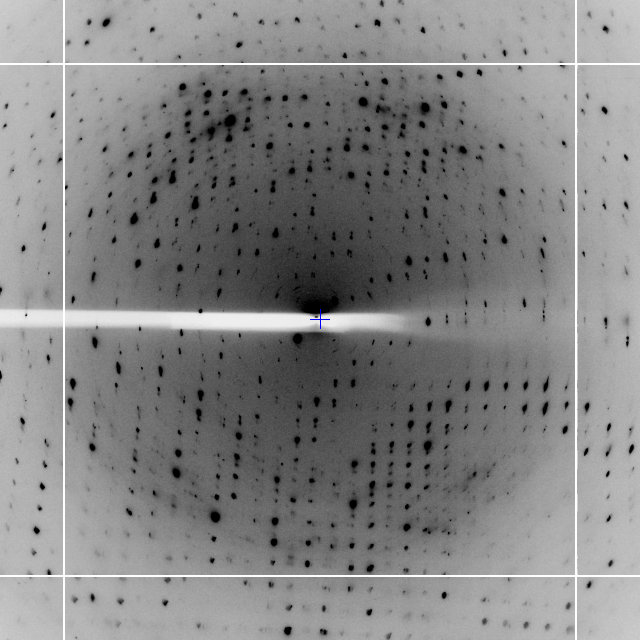
\includegraphics[scale=0.35]{figures/3qrn-diffraction.png}
\end{center}
\end{figure}

\begin{table}
\caption{Merging stats for the full data set for the example shown in
  the text.\label{table-merging-full}}
\begin{tabular}{lccc}
High resolution limit      &       1.25 &    6.45 &   1.25\\
Low resolution limit       &                18.85  & 18.85  &  1.27\\
Completeness               &                95.2   & 60.1  &  70.2\\
Multiplicity               &               12.2    & 8.4   &  4.8\\
I/sigma                    &               12.3    & 18.5   &  2.6\\
Rmerge                     &             0.113  & 0.096 &  0.564\\
Rmeas(I)                   &             0.129  & 0.118 &  0.633\\
Rmeas(I+/-)                &             0.121  & 0.105 &  0.679\\
Rpim(I)                    &             0.034  & 0.038 &  0.267\\
Rpim(I+/-)                 &             0.043  & 0.041 &  0.368\\
Wilson B factor            &            12.131& & \\
Anomalous completeness     &            93.3  &  52.6  &  58.0\\
Anomalous multiplicity     &           6.4    & 5.0  &   2.0\\
Anomalous correlation      &            0.544 &  0.791 & -0.297\\
Anomalous slope            &      1.085 &  0.000 &  0.000\\
Total observations         &       118588 & 529  &   1634\\
Total unique               &         9749  &  63 &     337\\
\end{tabular}
\end{table}

\begin{figure}
\caption{Merging statistics and completeness as a function of frame
  number for the example described in the
  text.\label{figure-rmerge-completeness}}
\begin{tabular}{cc}
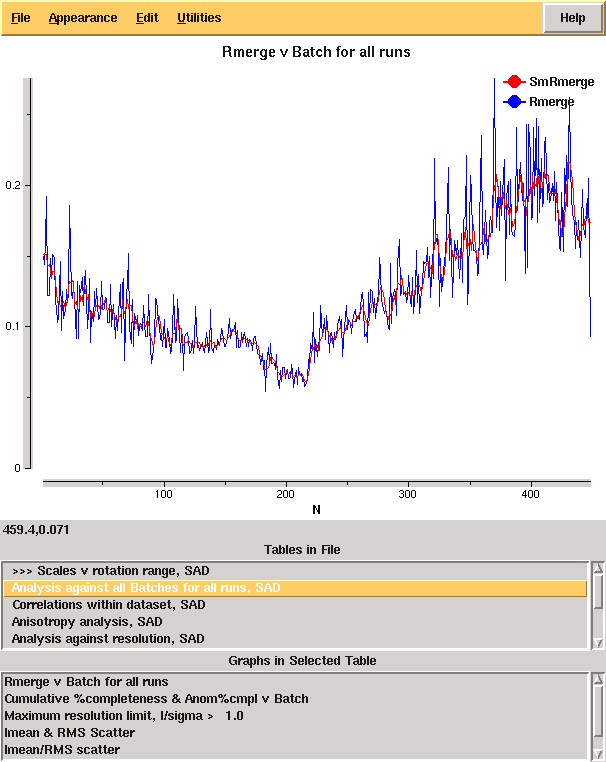
\includegraphics[scale=0.25]{figures/3qrn-all-rmerge-aimless.png} & 
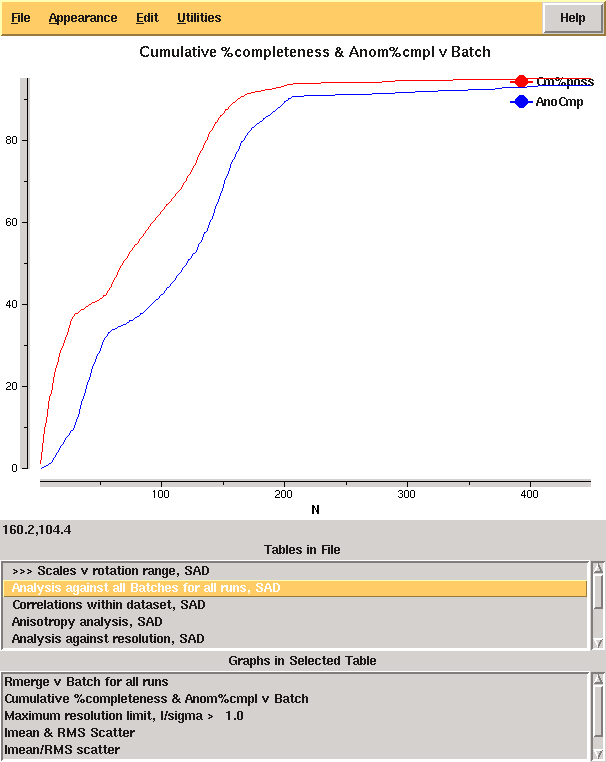
\includegraphics[scale=0.25]{figures/3qrn-all-complete-aimless.png} \\
\end{tabular}
\end{figure}

\subsection{Modifying input}

From the example it would seem sensible to investigate processing only the
first 200 of the 450 images. While it is usual to limit the batch range in 
scaling when processing the data manually, \emph{xia2} is not set up to 
work like this as decisions made for the full data set (e.g. scaling model
to use) may differ from those for the subset - we therefore need to rerun the
whole \emph{xia2} job after modifying the input. All that is necessary is to 
adjust the image range (START\_END) to get the modified input file shown in 
Figure~\ref{table-modified-xinfo} and rerun as 

\begin{verbatim}
xia2 -3d -xinfo modified.xinfo
\end{verbatim}

\noindent
giving the results shown in Table~\ref{table-merging-sub}. 
These are clearly much more internally
consistent and give nice results from experimental phasing though with
very poor low resolution completeness. At the same time 
we may wish to adjust the resolution limits to give more complete data in the 
outer shell, which may be achieved by adding a RESOLUTION instruction to 
either the SWEEP or WAVELENGTH block.

\begin{figure}
\begin{center}
{\small
\begin{verbatim}
BEGIN PROJECT AUTOMATIC
BEGIN CRYSTAL DEFAULT

BEGIN HA_INFO
ATOM Ba
END HA_INFO

BEGIN WAVELENGTH SAD
WAVELENGTH 0.979500
END WAVELENGTH SAD

BEGIN SWEEP SWEEP1
WAVELENGTH SAD
DIRECTORY /dls/i02/data/2011/mx1234-5
IMAGE K5_M1S3_3_001.img
START_END 1 200 ! THIS WAS 450
END SWEEP SWEEP1

END CRYSTAL DEFAULT
END PROJECT AUTOMATIC
\end{verbatim}
}
\end{center}
\caption{The modified input file to the program, showing the change to
START\_END.\label{table-modified-xinfo}}
\end{figure}

\begin{table}
\caption{Merging stats for the first 200 frames form the data set for
  the example shown in the text.\label{table-merging-sub}}
\begin{tabular}{lccc}
High resolution limit         &         1.22 &  6.34 &  1.22 \\
Low resolution limit          &        19.62 & 19.62 &  1.24 \\
Completeness                  &         86.9 &  49.1 &  37.8 \\
Multiplicity                  &        5.3  &  4.9   & 1.7 \\
I/sigma                       &        20.1 &  37.0  &  2.3 \\
Rmerge                        &       0.036 & 0.020  &0.355 \\
Rmeas(I)                      &       0.060 & 0.038  &0.448 \\
Rmeas(I+/-)                   &       0.043 & 0.023  &0.491 \\
Rpim(I)                       &       0.023 & 0.014  &0.297 \\
Rpim(I+/-)                    &       0.022 & 0.011  &0.339 \\
Wilson B factor               &       10.70& \\
Anomalous completeness        &        77.7  & 41.0  & 18.3 \\
Anomalous multiplicity        &         2.7  &  3.5  &  0.5 \\
Anomalous correlation         &        0.779 & 0.931 & 0.000 \\
Anomalous slope               &       1.553  &0.000 & 0.000 \\
Total observations            &       50875  &272   & 342 \\
Total unique                  &       9552   &55    & 199 \\
\end{tabular}
\end{table}

\section{Program Output}

As the program runs the key results are written to the screen and recorded
in the file \verb|xia2.txt|. This includes everything you should read and
includes appropriate citations for the programs that \emph{xia2} has used
on your behalf. There is also a file \verb|xia2-debug.txt| 
which should be send to 
xia2.support@gmail.com in the event of program failure. There are also two 
sensibly named directories, \verb|LogFiles| and \verb|DataFiles|, which will
be discussed shortly.

\subsection{xia2.txt}

In intention of the program output from \emph{xia2} is that it includes only
the information which is critical to read, as will be shown for a 450 image 
Pilatus 2M data set recorded from a Thaumatin crystal. Tthe results from 
indexing are displayed as lattice / unit cell:

{\small
\begin{verbatim}
------------------- Autoindexing SWEEP1 --------------------
All possible indexing solutions:
tP  57.60  57.60 149.51  90.00  90.00  90.00
oC  81.45  81.46 149.51  90.00  90.00  90.00
oP  57.59  57.60 149.50  90.00  90.00  90.00
mC  81.46  81.45 149.50  90.00  89.95  90.00
mP  57.60  57.59 149.53  90.00  89.93  90.00
aP  57.59  57.61 149.52  89.93  89.99  89.99
Indexing solution:
tP  57.60  57.60 149.51  90.00  90.00  90.00
\end{verbatim}
}

\noindent
where in each case the solution with the lowest penalty is displayed. The 
results of integration are displayed as one character per image - which 
allows the overall behaviour of the data to be understood at a glance. While
mostly 'o' is usually a good indication of satisfactory processing, '\%'
are not unusual, along with '.' for weaker data. If the output consists
of mostly 'O' then it may be helpful to record a low dose data set. The output
looks like:

{\small
\begin{verbatim}
-------------------- Integrating SWEEP1 --------------------
Processed batches 1 to 450
Weighted RMSD: 0.26 (0.09)
Integration status per image (60/record):
ooooooooooooooooooooooooooooooooooo.oooooooooooooooooooooooo
ooooooooooooooooooooooo.ooooooooooooooooooo.ooooooo.oooooooo
ooo.o.ooooooo.oooooooooooooooooooooooooooooooooooooooooooooo
oooooooooooooooooooooooooooooooooooooooooooooooooooooooooooo
oooooooooooooooooooo.ooooooooooooooooooooooooooooooooooooooo
ooooooooooooooooooooooooooooooooooooooooooooooooooo.oooooooo
ooooooooo.oooooooooo..ooo.oooooooooooooooooooo.ooooooooooooo
oooooooooooooooooooo.oooooooo.
"o" => good        "%" => ok        "!" => bad rmsd
"O" => overloaded  "#" => many bad  "." => blank
"@" => abandoned
Mosaic spread: 0.140 < 0.189 < 0.290
\end{verbatim}
}

\noindent
and includes a convenient legend.

\subsection{HTML pages}

If \verb|xia2html| has been run there is a nicely formatted html
version of this report, which includes graphical representation of
some of the log file output from e.g. Scala. Loading up
\verb|xia2.html| will give (hopefully self documenting) results as
shown in Figure~\ref{figure-xia2html}. If you have manually run xia2,
immediately running \verb|xia2html| in the same directory will generate this.

\begin{figure}
\caption{Illustration of xia2html output.\label{figure-xia2html}}
\begin{center}
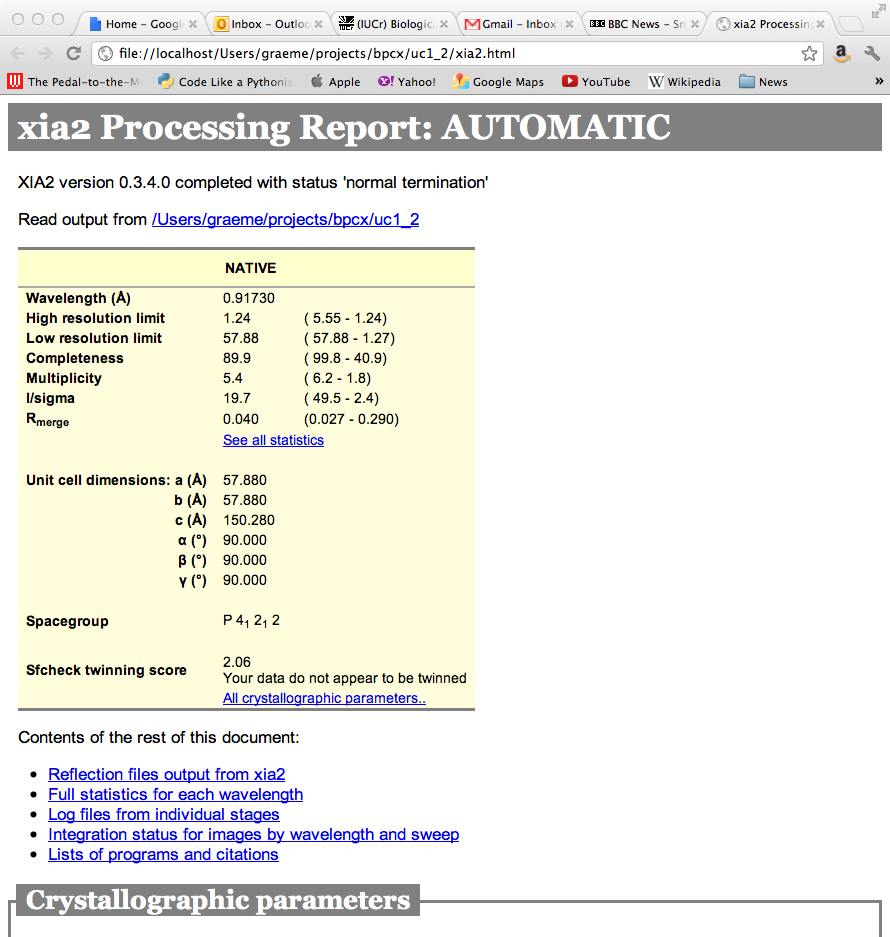
\includegraphics[scale=0.25]{figures/xia2html.png}
\end{center}
\end{figure}

\section{Commonly used program options}

There are a number of program options which are used on a daily basis in 
\emph{xia2}, which are:

\begin{center}
\begin{tabular}{|r|p{6cm}|}
\hline
-atom X & tell \emph{xia2} to separate anomalous pairs i.e. $I(+) \ne I(-)$ in 
scaling \\
-2d & tell \emph{xia2} to use MOSFLM and SCALA \\
-3d & tell \emph{xia2} to use XDS and XSCALE \\
-3dii & tell \emph{xia2} to use XDS and XSCALE, indexing with
    peaks found from all images \\
-2da & tell \emph{xia2} to use MOSFLM and AIMLESS \\
-3da & tell \emph{xia2} to use XDS and XSCALE, merging with AIMLESS \\
-3daii & tell \emph{xia2} to use XDS and XSCALE, merging with AIMLESS,
indexing with peaks found from all images \\
-xinfo modified.xinfo & use specific input file \\
-image /path/to/an/image.img & process specific scan \\
-spacegroup spacegroup\_name & set the spacegroup, e.g. P21 \\
-cell a,b,c,$\alpha$,$\beta$,$\gamma$ & set the cell constants \\ 
-small\_molecule & process in manner more suited to small molecule data \\
\hline
\end{tabular}
\end{center}

\noindent
Options running AIMLESS are able to cope with an extremely large
number of images, useful when trying to merge data from a number of
crystals each with a large number of images.

\subsection{Resolution limits}

The subject of resolution limits is one often raised - by default in
\emph{xia2} they are:

\begin{itemize}
\item{Merged $\frac{I}{\sigma_I} > 2$}
\item{Unmerged $\frac{I}{\sigma_I} > 1$}
\end{itemize}

\noindent
However you can override these with -misigma, -isigma.

\section{Installing xia2}

\emph{xia2} depends critically on having CCP4 and CCTBX
available. However to get access to the full functionality you will
also need XDS and Phenix (which includes Labelit and CCTBX.) Therefore
for a ``standard'' \emph{xia2} installation I would recommend:

\begin{itemize}
\item{Install CCP4 include updated versions of Pointless and Aimless
    from ftp://ftp.mrc-lmb.cam.ac.uk/pub/pre}
\item{Download XDS from http://xds.mpimf-heidelberg.mpg.de/ and
    add this to your path\footnote{To use -xparallel you will need to
      fiddle with forkintegrate in the XDS distribution}}
\item{Download PHENIX from http://www.phenix-online.org and be sure to
    source the setup for this \emph{after} CCP4}
\item{Download \emph{xia2} from http://xia2.sf.net and tweak the setup
    file to reflect where it's installed}
\end{itemize}

\noindent
By and large, if these instruction are followed you should end up with
a happy xia2 installation. If you find any problems it's always worth
checking the blog (http://xia2.blogspot.com) or sending an email to
xia2.support@gmail.com.

\section{Comments}

A question often asked is ``which options work best'' to which the
answer is always ``it depends!'' This is primarily because the outcome of
the analysis depends more on the quality of the data than anything
else. However I would always try for yourself and get a feel for how
the program works for your data - running both -2d and -3d will simply
require more computing time / disk space rather than more effort, so
it is certainly worthwhile. For small molecule data though -3dii
-small\_molecule is a good mix. Also -3d often works better for very
finely sliced data.

\section{Getting xia2}
\begin{itemize}
\item{Blog: xia2.blogspot.com}
\item{Code: xia2.sf.net}
\item{List: xia2-list@lists.sourceforge.net}
\end{itemize}

\end{document}
